\documentclass[%
10pt, %
final, % 
oneside, % 
onecolumn, %  
centertags]{article} % относится к классу article и размер шрифта 12 пунктовб, {article: статья, report: отчеты и диссертации, book: книга, letter: письмо}

% ------ page construction 

\topmargin= -30pt % насколько сверху будет страница
\textheight= 650pt

% ------ Пакеты расширения

\usepackage[utf8]{inputenc} % задает кодировку, utf-8 кодировка, включающая в себя знаки почти всех языков мира
\usepackage[english, russian]{babel} % подключает необходимые языки, основным языком является английский
\selectlanguage{russian} % настройки будут на английском, но писать будет на русском

\usepackage{euscript}
\usepackage{supertabular}

\usepackage[colorlinks=true,linkcolor=blue,unicode=true,urlcolor = blue]{hyperref} %hypered
\usepackage[pdftex]{graphicx} % для графики

\usepackage{amsthm, amssymb, amsmath, amsfonts} % математический пакет, математические шрифты
\usepackage{textcomp}
\usepackage[noend]{algorithmic}
\usepackage[ruled]{algorithm}
\usepackage{lipsum}
\usepackage{indentfirst}
\usepackage{babel}
\usepackage{pgfplots}
\usepackage{setspace}
\usepackage{xcolor}
\usepackage{hyperref}

\linespread{1.2} 
\setlength{\parindent}{2.4em}
\setlength{\parskip}{0.1em}

\pgfplotsset{compat=1.9}
\pgfplotsset{model/.style = {blue, samples = 100}} 
\pgfplotsset{experiment/.style = {red}}

\theoremstyle{plain}
\binoppenalty=10000

\newtheorem{theorem}{Теорема}[section] % theorem

\theoremstyle{definition}
\newtheorem{definition}{Определение}[subsection]

\theoremstyle{remark}
\newtheorem{remark}{Замечание}[section]

\newtheorem{corollary}{Следствие}

\newtheorem{proposition}{Proposition}

\newtheorem{example}{Пример}

\newtheorem{lemma}{Лемма}[section]

\renewcommand*{\proofname}{Proof}

\graphicspath{ {./images/} }


\begin{document}

\begin{titlepage} 
\begin{center}
\textbf{}\\[10.0cm]
\textbf{\LARGE Планирование расписаний и управление доходами}\\[0.5cm]
\textbf{\Large Александр Широков ПМ-1701} \\[0.2cm]


\begin{center} \large
{Преподаватель:} \\[0.5cm]
\textsc {Васильев Юрий Михайлович}\\
\end{center}

\vfill 



{\large {Санкт-Петербург}} \par
{\large {2020 г., 7 семестр}}
\end{center} 
\end{titlepage}

% Table of contents
\begin{thebibliography}{3}
  \bibitem{A}
\end{thebibliography}
\tableofcontents
\newpage

\section{Планирование расписаний и управление доходами}

\subsection{Задача из авиакомпании Россия}

В задачах планирования авиаперелетов:

\begin{itemize}
	\item расписание судов
	\item маршутизация
	\item построение графика полета летного состава
\end{itemize}

Мы поговорим о построении графика полета летного состава. Зарплата бортпроводника зависит от навыков и от некоторыз других факторов, но значительная часть денег тратилась на штрафы, которые выплачивались в пользу бортпроводников, потому что есть \textit{приказ}, о котором бортпроводник не может проводить в воздухе больше определенного времени в воздухе. 

Расписание в авиакомпании Россия делалось вручную и компания тратила много денег на выплаты бортпроводникам. OpenSky - программное обеспечение для обслуживания бортпроводников, но оно использовалось.

Множество борпроводников разбито на $4$ подмножеств с примерно одинаковыми характеристиками. Каждое подмножество называется \textbf{книга}.

\textbf{Рейс} - перелет из Петербурга в Москву, а \textbf{связка} - перелет из Петербурга в Мосвку и обратно. 

Множесто связок разбивалось на $4$ подмножества.

После этого соединяется первая книга и первый рейс и получается \textbf{рабочий стол}. Каждый рабочий стол можно описать характеристиками какими-то. С каждым рабочим столом работает один эксперт и все оказываются без перегрузов.

Задача: необходимо так разбить связки на подмножества, чтобы характеристики рабочих столов были примерно одинаковы.

\subsubsection{BiWay (ToWay) Number Partitional Problem}

Дано $n$ натуральных чисел и мультимножество (элементы могут повторяться) $S$, которое описывает этот набор $n$. Нам необходимо разбить подмножество $S=\{s_1,\ldots,s_n\}$ на два подмножества, каждое подмножество характерирузет сумму чисел, чтобы минимизировать максимальную сумму чисел в подмножестве.

\textbf{Greedy alghorytm}

\begin{enumerate}
	\item Отсортировать $S$ в порядке убывания
	\item На каждом шаге мы последовательно распределяем в две группы, кладём в группу с текущей наименьшей суммой. Если сумма одинакова, то кладем случайно.
\end{enumerate}

\textbf{Complete Greedy Alghorytm}

\begin{enumerate}
	\item Сортируем мультимножество в порядке убывания (распределяем большие числа и добиваем маленькими)
	\item Данный алгоритм исследует бинарное дерево, где каждому уровень - число из сортированного мультимножества, в каждой вершине - ветвление. В левой ветке - кладем в группу с наименьшей суммой, а в правой ветке - с наибольшей.
\end{enumerate}

Правила, позволяющие сократить размер нашего дерева:

\begin{itemize}
	\item Если сумма чисел в подмножествах равна, то мы кладем число только в одно подмножество
	\item Если оставшиеся распределенные числа не превосходят разницу между подмножествами, то мы кладем эти числа в группу с наименьшей суммой.
\end{itemize}

Домашнее задание: реализация алгоритма, причем настрока алгоритма в трех вариантах:
\begin{itemize}
	\item Исследует полное дерево решений и находит ответ;
	\item Алгоритм работает заданное число секунд и возвращает наилучший найденный результат за $t$ время (рекурсивная функция(оставшиеся числа, подмножества 1, подмножества 2))
	\item Первое найденное решение (первый лист, который мы нашли).
\end{itemize}

\textbf{Алгоритм Кармаркара-Карпа (эвристический)}

\begin{enumerate}
	\item Сортируем мультимножество в порядке убывания (распределяем большие числа и добиваем маленькими)
	\item Два наибольших числа заменяется на их разницу и кладём эту разницу в список с сортировкой и опять пересортировываем - кладем числа в два разных подмножества (интерпретация).

	\item Так делаем, пока не получим одно число: разницу межде максимальным и минимальным подмножеством
	\item Восстанавливаем
\end{enumerate}

Пример:
$$\{16,15,12,10,5,1\} \mapsto \{12,10,5,1,1\} \mapsto \{5,2,1,1\} \mapsto \{3,1,1\} \mapsto \{2,1\} \mapsto \{1\}$$

\textbf{Compete алгоритм Кармакара-Карпа}

\begin{enumerate}
	\item Сортируем мультимножество в порядке убывания (распределяем большие числа и добиваем маленькими)
	\item Исследуем бинарное дерево в глубину, исследуя левую ветку
\end{enumerate}

Домашнее задание: реализовать алгоритм для решения.

\subsubsection{MultiWay (ToWay) Number Partitional Problem}

Дано $n$ натуральных чисел и мультимножество (элементы могут повторяться) $S$, которое описывает этот набор $n$. Нам необходимо разбить подмножество $S=\{s_1,\ldots,s_n\}$ на $K$ подмножества, каждое подмножество характерирузет сумму чисел, чтобы минимизировать:
\begin{enumerate}
	\item минимизация максимальной суммы
	\item максимизация минимальной суммой
	\item минимизация разности между наибольшей и наименьшей суммой в подмножествах
	\item идеальная сумма - $\frac{S}{K}$ - минимизировать отклонения идеальной суммы
\end{enumerate}

$$X_{i,j} = \begin{cases}
	1, \text{if } S_i \text{ in } j \quad S_j \\
	0
\end{cases}$$

$$Z-W \to \min$$
$$\sum\limits_{j=1}^k X_{s,j}=1 \quad \forall s \in S$$

$Z$ - наибольшая сумма через $x$, а $W$ - наименьшую сумму через подмножества

$$Z \geq \sum\limits_{i=1}^n s_i X_{i,j} \quad \forall j \in \{1,\ldots,k\}$$
$$W \leq \sum\limits_{i=1}^n s_i X_{i,j} \quad \forall j \in \{1,\ldots,k\}$$
$$X_{i,j} \in \{0,1\}, \quad \forall i \in \{1,\ldots,n\}, \forall j \in \{1,\ldots,k\}$$

\textbf{Жадный алгоритм}

$L_j (S_1,S_2,\ldots,S_k,S_i)$

данная функция возвращает значение целевой функции, если мы положим число $S_i$ в $j$-е подмножество.

На каждом шаге алгоритма мы ищем такое $j \in \{1,\ldots,k\}$ такое, что значение целевой функции $gr = argmin L_j$ и так до тех пор пока мы не распределим все наши числа из отсортированного подмножества.
$$S_{gr} = S_{gr} \cup \{S_i\}$$

Программирование:

$c$ - список неизвестных, $m$ - коэффициенты при ограничениях, $\{\{const\},\{type\}\}$. Если $0$, то равенство, если $1$, то $\geq$, если $-1$, то $\leq$. 4-ый аргумент - интервалы, в которых могут применять значения неизвестные - $lbound, ubound$. Последний - какому множеству чисел принадлежит тип.

Домашнее задание: минимизация сумма отклонения по модулю от идеального разбиения и реализация.

$$\overline{y} = \frac{\sum S}{K}$$
$$\sum\limits_{i=1}^k |y_i - \overline{y}|$$

Линеаризация

\begin{itemize}
	\item Линеаризация модуля в ограничениях
	$$|X| \leq b (X=\sum\limits_{i=1}^n a_ix_i, b \geq 0)$$
	$$\begin{cases}
		x \leq b \\
		x \geq -b
	\end{cases}$$
	\item Допустимые значения
	$$x = 0 \text{ или } 0 \leq X \leq b, a >0$$
	$$y = \begin{cases}
		0, x=0 \\
		1
	\end{cases}$$
	$$\begin{cases}
		x \geq ay \\
		x \leq by \\
		y \in \{0,1\}
	\end{cases}$$

	\item Условие ИЛИ
	$$\sum\limits_{i=1} ^n c_ix_i \to \min$$
	$$\sum\limits_{i=1}^n a_{1,i}x_i \leq b_1 + M_1y$$
	$$\sum\limits_{i=1}^n a_{2,i}x_i \leq b_2+ M_2(1-y) \quad y \in \{0,1\}$$  
	\item Модуль со знаком $\geq$ 
	\item IF
	$$\text{if} \quad  \sum\limits_{i=1}^n a_{1,i}x_i \leq b_1 \to  \sum\limits_{i=1}^n a_{1,i}x_i \geq b_1 + \varepsilon$$
	$$\text{then} \quad \sum\limits_{i=1}^n a_{2,i}x_i \leq b_2 $$
	и мы превратили в третий пункт
	$$y \in \{0,1\}$$
	\item Умножение бинарных переменных
	$$\ldots + x_1\cdot x_2 + \ldots \leq b$$
	$$x_1,x_2 \in \{0,1\}$$
	$$y \in \{0,1\}$$
	$$y \leq x_1$$
	$$y \leq x_2$$
	$$y \geq x_1+x_2-1$$
	\begin{table}[H]
	\begin{center}
		\begin{tabular}{c|c|c|c|c} 
		$x_1$ & 1 & 0 & 0 & 0  \\ 
		$x_2$ & 1 & 0 & 1 & 0  \\ \hline
		$y$ & 1 & 0 & 0 & 0 
		\end{tabular}

	Линеаризация
	\end{center}
\end{table}
\end{itemize}

\subsection{Multi Dimensional Multi Way NPP}

Будем заниматься векторами. Минимизация максимальной разности по координатам между подмножествами.
$$1: (a_1,a_2,a_3)$$
$$2: (b_1,b_2,b_3)$$
$$3: (c_1,c_2,c_3)$$
$$\max (|a_1-b_1|, |a_2-b_2|,|a_3-b_3|) \to \min$$

Пусть $NC$ - размерность вектора, $NV$ - количество векторов, $NK$ - число групп.

Множество:
$$S = \{s_i \vert s_i = (s_{i,2},s_{i,2},\ldots,s_{i,NC})\}, i \in \{1,\ldots,NV\}$$
Неизвестные:
$$x_{s,k} = \begin{cases}
	1, - s \in NK \\
	0 
\end{cases}$$

Введем дополнительную переменную $y_{c,k}$ - сумма векторов из подмножества $k$ по координате $c$:
$$\max |y_{c,k_1} - y_{c,k_2}| \to \min$$
$$k_1,k_2 \in \{1,\ldots, NK\}$$
$$c \in \{1,\ldots,NC\}$$

Нам нужно найти группу $k_1,k_2$ и $c$ дают разницу по модулю между соответствующими $c$.

Так мы делаем для:
\begin{enumerate}
	\item $$\sigma \geq  y_{c,k_1} - y_{c,k_2}  \quad \forall k_1,k_2 \in \{1,\ldots,NK\}, k_1 < k_2$$
			$$\sigma \geq -y_{c,k_1} + y_{c,k_2} \quad \forall k_1,k_2 \in \{1,\ldots,NK\}, k_1 < k_2$$
			$$\sigma \to \min$$
	\item $$\sum\limits_{k=1}^{NK} x_{s,k} = 1, \qquad \forall s \in S$$ 
	\item $$y_{c,k} = \sum\limits_{s\in S} S_c \cdot x_{s,k} \forall c \in \{1,\ldots,NC\}, k \in\{1,\ldots,NK\}$$
	$$x_{s,k} \in \{0,1\} \forall s \in S, \forall k \in \{1,\ldots,NK\}$$

	Всего незивестынх: $NV*NK +1$
\end{enumerate}

\subsection{Рассмотрим взвешенную сумму средних квадратов отклонений}
$$\sum\limits_{k=1}^{NK}\sum\limits_{c=1}^{NC}w_c\left(1-\frac{y_{c,k}}{\hat{y}_c}\right)^2 \to \min$$
$\hat{y_c}$ - суммируем покоординатно $c$ и делим на $NK$ - идеальное значение по характеристике $c$ в подмножестве.

Чем больше $w_c$, тем больше значит тебя критерий равномерности - тем больше равны координатым векторов.

Такая запись нелинейна по $y$, то на дом будет модуль.

1-е ограничение нужно заменить на связь сигм с дельтами.

Усложним еще задачу.

\subsection{Критерий равномерности}

\begin{enumerate}
	\item Общее число ночных связок
	\item Среднее рабочее время на бортпроводника - берем подмножество связок, попавших на рабочий стол - суммируем время.
\end{enumerate}

Можем обобщить: что каждый вектор $S_{i,c,k}$ имеет разные координаты для разных подгрупп.

Приращение по характеристике $c$ при добавлении $i$ в $k$ подгруппе.
\newpage
\subsection{Minimize Differencse}

\textsc{Входные данные}: 
\begin{enumerate}
	\item $S$ - множество векторов
	\item $NV$ - мощность множества $S$
	\item $NC$ - размерность вектора $s \in S$, то есть каждый вектор описывается $NC$ числовыми координатами
	$$C = \{1,\ldots,NC\}$$

	Множество $S$ задаётся следующим образом:
	$$S = \{s_{i,1},s_{i,2},\ldots,s_{i,NC}\} \quad \forall i \in \{1,\ldots,NV\}$$
	\item $NK$ - число групп:
	$$K = \{1,\ldots,NK\}$$
\end{enumerate}
\textsc{Дополнение к входным данным}:
\begin{itemize}
	\item Введём дополнительную переменную $y_{c,k}$ - суммарное значение координаты $c \in C$ для группы $k \in K$.
\end{itemize}

\textsc{Задача:} необходимо распределить векторы из $S$ по $NK$ группам, причём каждый вектор должен быть представлен в единственной группе.

\textsc{Целевая функция:} минимизация максимальной разницы по модулю между двумя группами по координате среди всех координат и всех групп:
$$\underset{\underset{c\in C}{k_1,k_2\in K}}{\max} \left \vert y_{c,k_1} - y_{c,k_2} \right \vert \to \min$$

\textit{Пояснение:} необходимо найти две группы $k_1$ и $k_2$ и такую координату $c$, которые бы минимизировали максимальную разность.
\newpage
\textsc{Ограничения}:

\begin{enumerate}
	\item Каждый вектор должен находиться строго в одной из групп: 
	$$\sum\limits_{k=1}^{NK}x_{s,k} = 1 : \forall s \in S$$
	$$x_{s,k} \in \{0,1\}$$
	\item Сумма по каждой координате в каждой группе:
	$$y_{c,k} = \sum\limits_{s\in S} s_c \cdot x_{s,k}: \forall c \in C \  \forall k \in K$$
	\item Введём переменную $\sigma$, являющуюся максимальную разность по координате в группах. Её необходимо минимизировать:
	$$\sigma \to \min$$

	Введём ограничение, связывающую $\sigma$ и исходную целевую функцию:
	$$\left\vert y_{c,k_1} - y_{c,k_2} \right\vert \leq \sigma : \forall k_1,k_2 \in K \ \forall c \in C \ k_1 < k_2$$

	Модуль расскрывается через два неравенства:
	$$y_{c,k_1} - y_{c,k_2} - \sigma \leq 0$$
	$$-y_{c,k_1} + y_{c,k_2} - \sigma \leq 0$$ 
\end{enumerate}

Всего в задаче $NV\cdot NK + 1$ переменных.

\newpage

\subsection{Weighted Minimize}

\textsc{Входные данные}: 
\begin{enumerate}
	\item $S$ - множество векторов
	\item $NV$ - мощность множества $S$
	\item $NC$ - размерность вектора $s \in S$, то есть каждый вектор описывается $NC$ числовыми координатами
	$$C = \{1,\ldots,NC\}$$

	Множество $S$ задаётся следующим образом:
	$$S = \{s_{i,1},s_{i,2},\ldots,s_{i,NC}\} \quad \forall i \in \{1,\ldots,NV\}$$
	\item $NK$ - число групп:
	$$K = \{1,\ldots,NK\}$$
\end{enumerate}
\textsc{Дополнение к входным данным}:
\begin{itemize}
	\item Введём дополнительную переменную $y_{c,k}$ - суммарное значение координаты $c \in C$ для группы $k \in K$.
	\item Введём дополнительные \textsc{идеальные} константные значения следующим образом:
	$$\hat{y}_c = \frac{\sum\limits_{i=1}^{NV}s_{i,c}}{NK} : \forall c \in C$$
	\item Введём константы весов, отвечающие за значимость уравнивания по определенной координате - чем больше значение веса, тем важнее уравнивать множество по данной координате:
	$$W = \{w_1,\ldots,w_{NC}\}$$
\end{itemize}

\textsc{Целевая функция:} минимизация взвешенной ($W$) суммы модулей относительных отклонений $y_{c,k}$ от $\hat{y}_c$ по каждой из координат для каждой группы с учётом весов $W$:
$$\sum\limits_{c=1}^{NC} w_c \cdot \sum\limits_{k=1}^{NK} \left\vert 1 - \frac{y_{c,k}}{\hat{y}_c}\right\vert \to \min$$

\newpage
\textsc{Ограничения}:

\begin{enumerate}
	\item Каждый вектор должен находиться строго в одной из групп: 
	$$\sum\limits_{k=1}^{NK}x_{s,k} = 1 : \forall s \in S$$
	$$x_{s,k} \in \{0,1\}$$
	\item Сумма по каждой координате в каждой группе:
	$$y_{c,k} = \sum\limits_{s\in S} s_c \cdot x_{s,k}: \forall c \in C \  \forall k \in K$$
	\item Введём $NC\cdot NK$ переменных $\sigma[c,k]$, являющуюся верхней границей максимальной величины отклонения. Будем минимизировать сумму всех этих переменных:
	$$\sum\limits_{c=1}^{NC} w_c \cdot \sum\limits_{k=1}^{NK} \sigma[c,k] \to \min$$

	Введём следующие ограничения для относительных отклонений:
	$$\left\vert 1 - \frac{y_{c,k}}{\hat{y}_c}\right\vert \leq \sigma[c,k] : \forall c \in C \ \forall k \in K$$

	Модуль расскрывается через два неравенства:
	$$1 - \frac{y_{c,k}}{\hat{y}_c} - \sigma[c,k] \leq 0$$
	$$-1 + \frac{y_{c,k}}{\hat{y}_c} - \sigma[c,k] \leq 0$$ 
\end{enumerate}

Всего в задаче $NV\cdot NK + NC\cdot NK = NK(NV+NC)$ переменных.


\newpage
\subsection{Weighted Choose Minimize}

\textsc{Входные данные}: 
\begin{enumerate}
	\item $S$ - множество векторов
	\item $NV$ - мощность множества $S$
	\item $NC$ - размерность вектора $s \in S$, то есть каждый вектор описывается $NC$ числовыми координатами
	$$C = \{1,\ldots,NC\}$$
	\item $NK$ - число групп:
	$$K = \{1,\ldots,NK\}$$

	Координаты векторов могут отличаться в зависимости от попадания в подмножество, поэтому множество $S$ задаётся следующим образом:
	$$S = \{s_{i,k,1},s_{i,k,2},\ldots,s_{i,k,NC}\} \quad \forall i \in \{1,\ldots,NV\} \quad \forall k \in K$$
	
\end{enumerate}
\textsc{Дополнение к входным данным}:
\begin{itemize}
	\item Введём дополнительную переменную $y_{c,k}$ - суммарное значение координаты $c \in C$ для группы $k \in K$.
	\item Введём дополнительные \textsc{идеальные} константные значения следующим образом:
	$$\hat{y}_{c,k} = \frac{\sum\limits_{i=1}^{NV}s_{i,k,c}}{NK} : \forall c \in C \ \forall k \in K$$
	\item Введём константы весов, отвечающие за значимость уравнивания по определенной координате - чем больше значение веса, тем важнее уравнивать множество по данной координате:
	$$W = \{w_1,\ldots,w_{NC}\}$$
\end{itemize}

\textsc{Целевая функция:} минимизация взвешенной ($W$) суммы модулей относительных отклонений $y_{c,k}$ от $\hat{y}_{c,k}$ по каждой из координат для каждой группы с учётом весов $W$:
$$\sum\limits_{c=1}^{NC} w_c \cdot \sum\limits_{k=1}^{NK}  \left\vert 1 - \frac{y_{c,k}}{\hat{y}_{c,k}}\right\vert \to \min$$

\newpage
\textbf{\textsc{Ограничения.}}:

\begin{enumerate}
	\item Каждый вектор должен находиться строго в одной из групп и вектор из группы возможных векторов в зависимости от номера группы должен быть тоже один.
	$$\sum\limits_{i=1}^{NK} \sum\limits_{k=1}^{NK}x_{s,i,k} = 1 : \forall s \in S $$
	$$x_{s,i,k} \in \{0,1\}$$

	Количество переменных: $NV\cdot NK^2$
	\item Сумма по каждой координате в каждой группе:
	$$y_{c,k} = \sum\limits_{i=1}^{NK} \sum\limits_{s\in S} s_{i,c} \cdot x_{s,i,k}:  \forall c \in C \  \forall k \in K $$
	\item Введём $NC\cdot NK$ переменных $\sigma[c,k]$, являющуюся верхней границей максимальной величины отклонения. Будем минимизировать сумму всех этих переменных:
	$$\sum\limits_{c=1}^{NC} w_c \cdot \sum\limits_{k=1}^{NK} \sigma[c,k] \to \min$$

	Введём следующие ограничения для относительных отклонений:
	$$\left\vert 1 - \frac{y_{c,k}}{\hat{y}_{c,k}}\right\vert \leq \sigma[c,k] : \forall c \in C \ \forall k \in K$$

	Модуль расскрывается через два неравенства:
	$$1 - \frac{y_{c,k}}{\hat{y}_{c,k}} - \sigma[c,k] \leq 0$$
	$$-1 + \frac{y_{c,k}}{\hat{y}_{c,k}} - \sigma[c,k] \leq 0$$ 
\end{enumerate}

Всего в задаче $NV\cdot NK^2 + NC \cdot NK = NK\cdot(NV \cdot NK + NC)$ переменных.

\newpage
\subsection{Натурные данные 16.09.2020}

\textsc{Входные данные}: 

Книга - подмножество бортпроводников. Подмножества связок должны быть примерно одинаковым.

Пусть $M$ - количество связок, выданных на месяц. 

$F = \{f_1,\ldots,f_m\}$ - множество оборотных рейство (оборотный рейс и связки - одно и тоже).

$M' < M$  - число ночных связок - ночной связкой считается та связка, 50 процентов её рейсов относится с $22:00$ до $6:00$.

\textbf{\textsc{Характеристики связки $f \in F$.}}
\begin{itemize}
	\item $t_f$ - время воздушного судна в воздухе - время налёта
	\item $p_f$ - размер экипажа - сколько борпроводников должно назначиться на связку $(3,4)$
	\item $v_f$ - тип сообщения (ВВЛ, МВЛ, СНГ) - внутренняя воздушая линия, международная воздушная линия, союз независимых государств
	\item $U_1$ - множество связок ВВЛ, $u_1'$ - множество ночных связок ВВЛ
	\item $U_2$ - множество связок МВЛ, $u_2'$ - множество ночных связок МВЛ
	\item $U_3$ - множество связок СНГ, $u_3'$ - множество ночных связок СНГ
	
	$U_{\alpha}' < U_{\alpha}, \forall \alpha \in \{1,2,3\}$
	\item $d_f \in T$ - дата вылета (дата начала связки) - множество дней горизонта планирования
	\item $a_f \in L$ - тип воздушего судна (ВС), на котором осуществляется связка, $L$ - множество типов ВС

	\item $A_l, l \in L$ - множество связок с типом воздушного судна -  $l$
	\item $s_f$ - направление связки - тот город, куда направляется из Санкт-Петербурга $s_f \in R$, $R$ - множество всех направлений
	\item $D_i$ - множесво связок с вылетом в день $i$
\end{itemize}

\textbf{\textsc{Книги.}}:

$B = \{B_1,\ldots,B_k\}$ - $K$ подмножеств бортпроводников, $B$ - множество книг, каждая книга характеризуется $3$ характристиками:
$$c_{\alpha,k}; \forall \alpha \in \{1,2,3\}; \forall k \in \{1,\ldots,K\}$$

$c_{1,k}$ - число доступных бортпроводников в группе $K$, из множества ВВЛ для планирования

$c_{2,k}$ - число доступных бортпроводников в группе $K$, из множества МВЛ для планирования

$c_{3,k}$ - число доступных бортпроводников в группе $K$, из множества СНГ для планирования

Необходим разбить подмножество связок на $K$ подмножеств, с учётом критериев равномерности.

\textbf{\textsc{Критерий равномерности.}}

\begin{enumerate}
	\item Средний налет на одного бортпроводника по типу сообщения (включает в себя $3$ характеристики по ВВЛ, МВЛ, СНГ)

	Пусть $\hat{y}_{j,k}$ - это усреднённое значение $j$-ой характеристики $k$-ой группы. Введем три идеальных значения:
	$$\hat{y}_{j,k} = \frac{\sum\limits_{i \in U_j} p_i \cdot t_i}{\sum\limits_{k'=1}^K c_{j,k'}}; \forall j \in \{1,2,3\}; \forall k \in \{1,\ldots,K\}$$
	равен сумме налета по каждой связки из соответствующего типа сообщения, деленное на суммарное число бортпроводников по каждому типу сообщения 
	\item Средний ночной налёт на одного бортпроводника по типу сообщения:
	$$\hat{y}_{3+j,k} = \frac{\sum\limits_{i \in U_j'} p_i \cdot t_i}{\sum\limits_{k'=1}^K c_{j,k'}}; \forall j \in \{1,2,3\}; \forall k \in \{1,\ldots,K\}$$
	\item Общее число ночных связок на рабочих столах (РС) пропорционально числу бортпроводников на рабочем столе - чем больше бп на рабочем столе, тем больше ночных связок на рабочем столе:
	$$\hat{y}_{7,k} = \frac{c_{1,k}\cdot M'}{\sum\limits_{k'=1}^K c_{j,k'}}; \forall k \in\{1,\ldots,K\}$$
	\item Общее число связок по типу сообщения для рабочего стола (РС) должно быть пропорционально числу бортпроводников, доступных для планирования по типу сообщения:
	$$\hat{y}_{7+j,k} = \frac{c_{j,k}\cdot \vert U_j\vert}{\sum\limits_{k'=1}^K c_{j,k'}}; \forall j \in \{1,2,3\};\forall k \in\{1,\ldots,K\}$$
	\item Равенство общего количества связок в день для рабочего стола (РС) (каждый день эксперты должны следить за примерно одинаковым количеством бортпроводником и не было перегруза в сторону какого-то эксперта):
	$$\hat{y}_{10+j,k} = \frac{\vert D_j \vert}{K}; \forall j \in \{1,\ldots,\vert T \vert\};\forall k \in\{1,\ldots,K\}$$
	\item Общее количество связок по типу воздуных судов (ВС) для рабочего стола (РС):
	$$\hat{y}_{10+\vert T \vert + j, k} = \frac{\vert A_j \vert}{K}; \forall j \in \{1,\ldots,\vert L \vert\}; \forall k \in \{1,\ldots,K\}$$
	\item Общее количество связок по направлению для РС. $S_i$ - множество связок по направлению:
	$$\hat{y}_{10+\vert T \vert + \vert L \vert + j, k} = \frac{\vert S_j \vert}{K}; \forall j \in \{1,\ldots,\vert R \vert\}; \forall k \in \{1,\ldots,K\}$$

	Размерность идеального вектора для группы:
	$$N = 10 + \vert T \vert + \vert L  \vert+ \vert R \vert$$
\end{enumerate}

Для любой связки $f \in F$ введем следующие матрицы:
$$\Delta f =  \{\delta_{f,j,k}\}_{j \in \{1,\ldots, N\};k \in \{1,\ldots,K\}}$$
где $\delta_{f,j,k}$ - приращение $j$-ой характеристики при распределении $f$-ой связки в группу $k$ - описание вектора для описания в предыдущей задачи.

$\Large \Delta = \{\Delta_1,\Delta_2,\ldots,\Delta_m\}$ - тензор приращений.

$\Delta_{f,k}$ - вектор (столбец) значений приращений при добавлении $f$-ой связки в $k$-ую подгруппу.

\textbf{Целевая функция.}
$$\sum\limits_{k=1}^K \sum\limits_{j=1}^N w_j \left(1- \frac{y_{j,k}}{\hat{y}_{j,k}}\right )^2 \to \min$$


Веса характеристик, принадлежащим одному критерию, равны (веса для первых трех характеристик равны). $7$ критериев, описывается $3$-мя характеристиками, веса для этих характеристик равны.

\textbf{Решение задачи.}

2135 связок и 6 групп, то мы не можем решить целочисленным программированием. Решим задачу с помощью жадного алгоритма:


\textbf{Алгоритм 1.}

Пусть $L$ - функция работает от $k$ аргументов. Каждый аргумент описывает характеристики $k$-го подмножества $j = \{1,\ldots,N\}$
$$L(y_1,\ldots,y_K) = \sum\limits_{k=1}^K \sum\limits_{j=1}^N w_j \cdot \left(1-\frac{y_{j,k}}{\hat{y}_{j,k}}\right)^2$$
где $y_i = (y_{1,i},\ldots,y_{N,i})$.

На шаге $\textsc{step}$ мы ищем такую пару $k$ и $f$, чтобы минимизировать значение целевой функции. На каждом шаге распределяем одну связку в одно из подмножеств.
$$L_k(y_1,\ldots,y_K,f) = L(y_1',y_2',\ldots,y_k')$$
где
$$y_i' = \begin{cases}
	y_i, \operatorname{if} i \neq k \\
	y_i + \Delta_{f,i}
\end{cases}; \forall i \in \{1,K\}$$
будет искать такую связку, при котором значении функции минимально.

Введем $y_k = (0,\ldots,0)$, $k \in \{1,\ldots,K\}$:

Пока $F \neq 0$ ищем $(k,f) = \underset{k \in \{1,\ldots,K\}, f \in F}{\operatorname{argmin}} L_k(y_1,\ldots,y_K,f)$

Мы нашли связку $f$ маленькую, поэтому мы можем вычеркнуть ее из связок:
$$F = F \\ \{1\}$$
$$y_k = y_k+ \Delta_{f,k}$$

и сохраняет, что $f$ в $k$. Цикл заканчивается и выдается распределение.

\begin{itemize}
	\item Выбираем $K \cdot M$ вариантов - в какую группу положить связку
	\item Выбираем $K \cdot (M-1)$
\end{itemize}

\textbf{Алгоритм 2. С сортировкой связок}

\textbf{nb document.}

\begin{enumerate}
	\item Импорт исходных файлов + эксперт
	\item Позволяет вводить веса критериев
	\item Позволяет проводить расчеты по A1 и A2 (2 типа сортировки)
	\item Создавать отчет по результатам по результате работы алгоритма
	\begin{itemize}
		
		\item Средний налет на бортпроводника - Последняя строка - максимальная разность по модулю между значениями в столбце - максимум по минимум
	\end{itemize}
	\item Функционал для сравнения результатов работ алгоритмов + решение эксперта
\end{enumerate}

\subsection{Метод Сугиямы}

1) Поиск такого максмимального аиклического подграфа. Дан $G = (V, A) \to G' \leq G: v' = (V, A')$, $|A'| \to \max$

2) Минимальный feedback arc set:
$$G = (V, A) \to FASCA, G'' = (V, A \backslash FAS)$$

3) Минимальный Feedback Set:
$$G = (V, A) \to FS \subset A, G'' = (V, (A \backslash FS) \cap rev(FS))$$
ацикличнское, $|FS| \to \min$

\subsection{Set Covering Formulation}

Дан ориентированный граф. Нужно минимальный взвешенный Feedback Set, максимальный вес ацикличного подграфа.
$$y_{i,j} = \begin{cases}
	1, (i,j) \in FAS \\
	0, \text{если не удаляем}
\end{cases}$$

Матрица $M (c\times n)$, где $m_{i,j} = 1$, если дуга под номером $j$ в цикле $i$.

Мощность $|A| = n$, $C$ - количество циклов в графе. Использовать FindCycles

$$\sum\limits_{(i,j) \in A} w_{i,j} \cdot y_{i,j} \to \min$$

Из цикла нужно удалить как минимум одну дугу. МЫ проходимся по всем циклам от $\forall i \in \{1, \ldots, c\}$

$$\sum\limits_{j=1}^n m_{i, j}y_{A(j)} \geq 1$$
где $A(j)$ - это $j$-ая дуга из $A$. 

Формируем количество переменных $y $по количеству дуг. Формируем матрицу $M$. Результатом является минимальный FAS -> FS.

\newpage
\subsection{Неравенство Треугольника}
\label{nerav}
Найти такой порядок вершин, чтобы при линейной укладке как можно меньше дуг смотрело справа налево, суммарный вес дуг наименьший. Дуги с наименьшим весом - менее важны.

Пусть дан граф $G = (V, E)$, $n$ - количество рёбер: $\#E$

Пусть $\pi$ - перестановка в лексикографическом порядке вершин (по возрастанию от $1,\ldots, n$). Сформируем матрицу \(C \in \mathbb{R}^{n \times n}\), элементами которого будут $c_{i,j}$, такие, что:
$$c_{i,j} = \begin{cases}
	w_{i,j}, (i,j) \in A\\
	0
\end{cases}$$
что означает, что мы заполняем вес ребра в матрицу, если оно есть в рёбрах графа.

Введём переменные задачи:
$$x_{i,j} = \begin{cases}
	1,\  \pi^*(i) < \pi^*(j): \  \forall i, j \in V, \pi(i) < \pi(j)\\
	0
\end{cases}$$
что означает, что мы будем брать те переменные, которые равны $1$, то есть стоят левее в линейной укладке. Всего у нас порядка $O(n^2)$ переменных, а именно $\frac{n(n-1)}{2}$.

Целевая функция задачи разбивается на две суммы:
$$\sum\limits_{\underset{\pi(j)>\pi(i)}{j,i \in E}}c_{i,j}x_{i,j} + \sum\limits_{\underset{\pi(i)<\pi(j)}{i,j \in E}}c_{i,j}(1-x_{i,j}) \to \min$$
что означает, что в первой сумме суммируются все дуги у который первая вершина больше второй в лексикографическом порядке, а во второй - те дуги, у которых первая вершина меньше второй в лексикогафическом порядке.

Ограничения:
$$0 \leqslant x_{i,j} + x_{j,k} - x_{i,k} \leqslant 1, \forall i,j,k \in V, \pi(i)< \pi(j) < \pi(k)$$
$$x_{i,j} = \{0,1\}, 1 \leqslant i,j \leqslant n$$

\newpage
\subsection{Layering}

Пусть дан ациклический ориентированный граф $G = (V,A)$, необходимо разбить на слои $V_1, V_2,\ldots, V_k$, чтобы $\forall (u, v) \in A: u \in V_i, v \in V_j, i<j$. Введём переменные $\lambda(u)$. Целевая функция:
$$\sum\limits_{(u,v)\in A}(\lambda(v) - \lambda(u)) \to \min$$

Ограничения:
$$\lambda(v) - \lambda(u) \geqslant 1 \quad \forall (u,v) \in A$$
$$\lambda(v) \geqslant 1 \quad \forall v \in V$$
$$\lambda(u) \in \mathbb{Z} \quad \forall v \in V$$ 

\newpage
\subsection{Распределение вершин по слоям с ограничением на ширину слоя}

Пусть дан $G(V, A)$ - DAG (Directed Acyclic Graph). Решается задача распределения по слоям. Введём следующие переменные:
$$X_{i, k} = \begin{cases}
	1, \text{если вершина \textbf{i} назначена на слой \textbf{k}}\\
	0, \text{в обратном случае}
\end{cases}$$

Обозначим за $W$ - максимальную ширину слоя, за $n_v$ - число вершин в графе. Тогда ограничение:
$$\sum\limits_{i=1}^{n_v} X_{i, k} \leqslant W \quad \forall k \in \{1, \ldots, h_{\max}\}$$
где $h_{\max}$ - длина наибольшего пути в графе. Данное ограничение означает, что количество вершин на каждом слое не может превышать $W$.

Для каждой вершины $i \in V$ определим минимальный и максимальный номер слоя, на котором может располагаться вершина $i$:
$$[\ \underline{h_i},  \ \overline{h_i}\ ] \quad \forall i \in V$$

тогда количество переменных уменьшится:
$$X_{i, k} = \begin{cases}
	1, \text{если вершина \textbf{i} назначена на слой \textbf{k}}\\
	0, \text{в обратном случае}
\end{cases}, \underline{h_i} \leqslant k \leqslant \overline{h_i} $$
$$X_{i, k} \in \{0,1\}$$
$$\forall i \in V \quad \forall k \in \{\underline{h_i}, \overline{h_i}\}$$

Номер слоя вершины $\forall i \in V$ вычисляется следующим образом:
$$\lambda(i) = \sum\limits_{k = \underline{h_i}}^{\overline{h_i}} k \cdot X_{i, k}$$

Ограничение: каждая вершина назначается ровно на один слой:
$$\sum\limits_{k = \underline{h_i}}^{\overline{h_i}} X_{i, k} = 1$$

Ограничение, что направление дуг - сверху вниз:
$$\lambda(v) - \lambda(u) \geqslant 1 \quad \forall (u,v) \in A$$
$$\sum\limits_{k = \underline{h_i}}^{\overline{h_i}} k \cdot X_{v, k} - \sum\limits_{k = \underline{h_i}}^{\overline{h_i}} k \cdot X_{u, k} \geqslant 1 \quad \forall (u,v) \in A$$

Теперь переходим к главному: целевая функция. Необходимо минимизировать число фиктивных вершин. Для этого воспользуемся логическим рассуждением: чем меньше слоёв нам потребуется для расстановки вершин по слоям, тем меньшее количество фиктивных вершин будет в Layering графе. Поэтому введём переменную $\Phi$ и будем ёё минимизировать при дополнительном ограничении:
$$\Phi \to \min$$
$$\lambda(i) = \sum\limits_{k = \underline{h_i}}^{\overline{h_i}} k \cdot X_{i, k} \leqslant \Phi \quad \forall i \in V$$

Если $W$ - переменная, то введём веса и целевая функция примет вид:
$$w_1 \cdot \Phi + w_2 \cdot H \to \min$$

\newpage
\subsection{Гиперграф}

Для начала разберёмся, что такое гиперребро. Гиперребро задаётся с помощью двух понятий: \textsc{источник} и \textsc{множество стоков} - вершин, соедиённых с источником. Так же у нас есть понятие \textsc{горизонтального сегмента} - прямая, соединяющая стоки.

Далее у нас есть $3$ вида пересечений:

\begin{enumerate}
	\item горизонтальный сегмент пересекает линию от источника
	\item горизонтальный сегмент пересекат сток
	\item стоки накладываются друг на друга
\end{enumerate}

Все это представлено на картинке ниже:

\begin{center}
	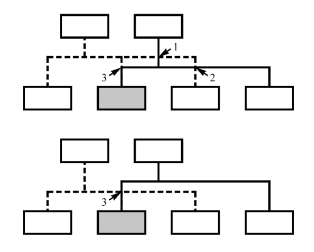
\includegraphics[scale=0.8]{1.png}

 	Рис.1 Три вида пересечений
\end{center}

Дан двухслойный гиперграф $H_2 = (V_1, V_2, E_{H_2})$, где $V_1 = \{u_1, \ldots, u_{N_1}\}$ и $V_2 = \{v_1, \ldots, v_{N_2}\}$ - множество вершин верхнего и нижнего слоя, а $E_{H_2}$ - множество одноисточных рёбер. Для каждой вершины $v \in V_1 \cup V_2$ двухслойного гиперграфа известны координаты $x(v), y(v)$.

\textbf{Алгоритмы минимиации числа пересечений гиперёбер}

Введём $8$ видов целочисленных переменных:

1. Переменные $Z_i'$ и $Z_j''$ характеризуют количество единичных сдвигов вершин верхнего $u_i \in V_1$ и нижнего слоя $v_j \in V_2$, знаки определяют направление сдвигов.

Новые абсциссы вершин $u_i \in V_1, v_j \in V_2$ будут равны:
$$x'(u_i) = x(u_i) + \Delta \times Z_i' \eqno (1.1.1)$$
$$x'(v_j) = x(v_j) + \Delta \times Z_j'' \eqno (1.1.2)$$

2. Переменные $AZ_i'$ и $AZ_j''$ - это количество единичных сдвигов вершин $u_i$ и $v_j$, соответственно, то есть:
$$AZ_i' = \vert Z_i'\vert \eqno (1.2.1)$$
$$AZ_j'' = \vert Z_j''\vert \eqno (1.2.2)$$

3. Для каждой пары гиперрёбер $(e_n, e_m)$, где $e_n = (u_{\eta}, T_{\eta}), e_m = (u_{\mu}, T_{\mu})$ и первый источник находится левее второго источника гиперребра ($x(u_{\eta}) < x(u_{\mu})$) задаются следующие переменные:
$$HH_{n, m} = \begin{cases}
	0, \text{если горизонтальный сегмент } e_m \text{ \textbf{выше}, чем } e_n \\
	1, \text{если горизонтальный сегмент } e_m \text{ \textbf{ниже}, чем } e_n
\end{cases} \eqno (1.3.1)$$
$$CT1_{n, m} = \begin{cases}
	0, \text{горизонтальный сегмент \textbf{не пересекает} линию от источника} \\
	1, \text{горизонтальный сегмент \textbf{пересекает} линию от источника}
\end{cases} \eqno (1.3.2)$$
$$CT2_{n, m} = \begin{cases}
	c_{e_n, e_m}, \text{если горизонтальный сегмент } e_m \text{ \textbf{выше}, чем } e_n \\
	c_{e_m, e_n}, \text{если горизонтальный сегмент } e_m \text{ \textbf{ниже}, чем } e_n
\end{cases} \eqno (1.3.3)$$
где $c_{e_n, e_m}$ - количество пересечений второго типа между гиперрёбрами $e_n$ и $e_m$ в зависимости от взаимного расположения горизонтальных сегментов.

4. Переменные $BV_{\eta, j}$ - это булевы фиктивные переменные, которые сводятся для каждого гиперребра $e_n = (u_{\eta}, T_{\eta})$ и для таких вершин $v_j$ нижнего слоя, не смежных вершине $u_{\eta}$.

\textbf{Целевая функция минимизации пересечений гиперрёбер}

Выбор целевой функции задачи целочисленного программирования обусловлен целями:

\begin{itemize}
	\item минимиация пересечений первого и второго типа
	\item минимизация сдвигов вершин
\end{itemize}

В терминах нашей задачи:
\begin{itemize}
	\item Количесвто единичных сдвигов для вершин первого уровня должно быть как можно меньше
	$$\sum\limits_{i=1}^{\vert V_1 \vert}AZ_i'$$
	\item Количество единичных свдигов для вершин второго уровня должно быть как можно меньше
	$$\sum\limits_{j=1}^{\vert V_2 \vert}AZ_j''$$
	\item Число пересечений и второго типа:
	$$\sum\limits_{n=1}^{\vert E_{H_2}\vert - 1}\sum\limits_{m=n+1}^{\vert E_{H_2} \vert}CT1_{n,m} + CT2_{n,m}$$
\end{itemize}

Очевидно, что все этир критерии берутся с какими-то весами, поэтому целевая функция будет выглядеть следующим образом:
$$L = w_z \cdot \left(\sum\limits_{i=1}^{\vert V_1 \vert}AZ_i' + \sum\limits_{j=1}^{\vert V_2 \vert}AZ_j''\right) + \sum\limits_{n=1}^{\vert E_{H_2}\vert - 1}\sum\limits_{m=n+1}^{\vert E_{H_2} \vert} w_{c_1} \cdot CT1_{n,m} +w_{c_2} \cdot  CT2_{n,m} \to \min \eqno (1)$$

Теперь запишем ограничения:

\textsc{Ограничение 2-3:}
\begin{center}
	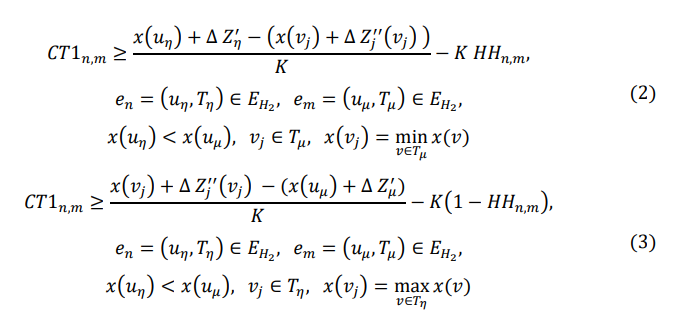
\includegraphics[scale=0.6]{2.23.png}
\end{center}

\textbf{Объяснение}: было объяснено на паре, но суть следующая: $x(v_j) = \underset{v \in T_{\mu}}{\min} x(v)$ означает, что данная вершина наиболее левая вершина для первого слоя, а в третьем ограничении - что наиболее правая дл второго слоя. Тогда если \text{если горизонтальный сегмент } $e_m$ \text{ \textbf{выше}, чем } $e_n$, то $HH_{n, m} = 0$, то второе утверждение говорит нам, что вершина $u_{\theta}$ имеет новые координаты абсцисс левее, чем вершниа $v_j$. При подстановке $HH_{n,m} = 1$ все в точности наоборот.

\textsc{Ограничение 4-5:}
\begin{center}
	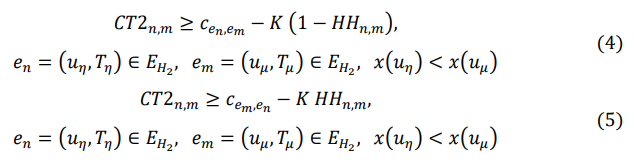
\includegraphics[scale=0.6]{2.45.png}
\end{center}

\textbf{Объяснение}: \text{если горизонтальный сегмент } $e_m$ \text{ \textbf{выше}, чем } $e_n$, то $HH_{n,m} = 0$, $CT_2 = c_{e_n, e_m}$, ограничение $4$ принимает вид: $0 \geqslant -K$, а $(5)$ - $CT2_{n,m} \geqslant c_{e_m, e_n}$ - устанавливаем ограничение на число пересечений второго типа а при обратном $HH_{n,m} = 1$ и $4$-е ограничение просто выполняется всегда.

\textsc{Ограничение 6-9:}
\begin{center}
	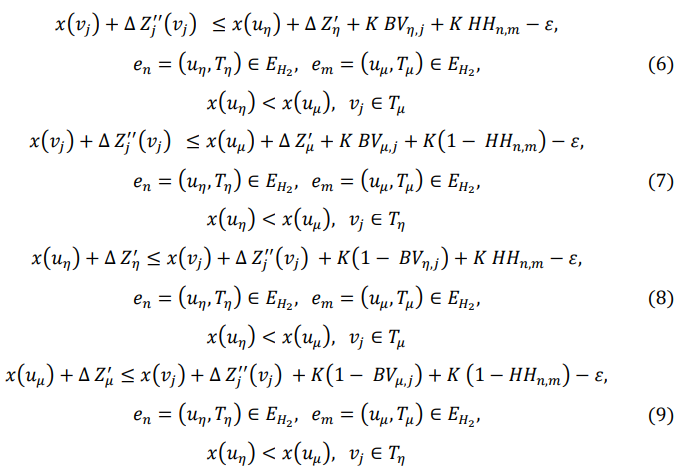
\includegraphics[scale=0.6]{2.69.png}
\end{center}

\textbf{Объяснение}: в данных огарничениях у нас есть координатs абсцисс новых вершин $v_j$ и $\mu_{\eta}$. При подстановке различных значений переменных $HH_{n, m}$, \text{если горизонтальный сегмент } $e_m$ \text{ \textbf{выше}, чем } $e_n$, то мы пытаемся задать расположение рёбер и всё зависит от булевых фиктивных вершин, не смежных $u_{\eta}$. Если фиктивная переменная равна единице, то для ограничения $6$ это означает, что $v_j$ находится правее $v_j$, так как мы должны добавить какую-то константу $K$, а если $0$, то левее. Далее с другими ограничениями аналогично. Но вообще я запутался с этим, мне не очень понятно. С переменными понимаю вроде смысл, а ограничений нет..

\textsc{Ограничение 10-11:}
\begin{center}
	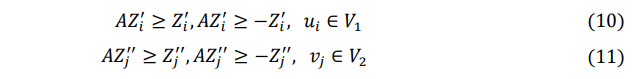
\includegraphics[scale=0.6]{2.1011.png}
\end{center}

\textbf{Объяснение}: это просто линеаризация модуля из формул $(1.2.1)$ и $(1.2.2)$ и для целевой функции $(1)$.

\textsc{Ограничение 12-13:}
\begin{center}
	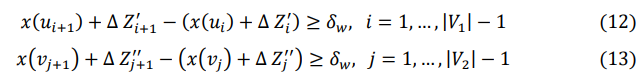
\includegraphics[scale=0.6]{2.1213.png}
\end{center}

\textbf{Объяснение}: для каждой вершины разница в новых абсциссах между правым её соседом и самой вершины на первом слое больше какого-то значения $\delta_w$. То же самое и для вершин второго слоя.

\textsc{Ограничение 14:}
\begin{center}
	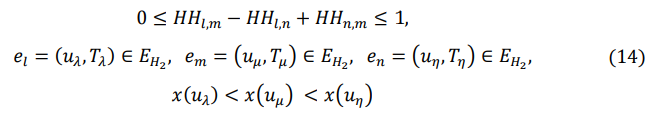
\includegraphics[scale=0.6]{2.14.png}
\end{center}

\textbf{Объяснение}: пусть у нас есть $3$ гиперребра и первое гиперребро левее всех остальных ребер, а второе левее третьего. Тогда по сути это неравенство треугольника для горизонтальных сегментов в высоту - задает порядок для каждой тройки гиперрёбер в высоту: либо горизонтальный сегмент выше, чем другие и тогда все нули, либо выше тогда, все единицы и.т.д.


\textbf{Алгоритм решения задачи минимизации числа пересечений гиперребер через задачу поиска линейной укладки}

Одним из подходов к решению задачи минимизации числа пересечений гиперребер является ее формулировка в
виде задачи устранения циклов в некотором взвешенном направленном графе. Каждая вершина этого графа
соответствует горизонтальному сегменту гиперребра, и каждая пара вершин соединена двумя противонаправленными
взвешенными дугами. Направление дуги показывает, какая вершина (т.е. соответствующий ей горизонтальный
сегмент) расположена выше, а ее вес определяется взвешенной суммой числа пересечений и недопустимых наложений
гиперребер, соответствующих вершинам.

Буду ссылаться на алгоритм неравенства треугольника из пункта 1.11 в линейной укладке графа, который мы проходили со страницы \pageref{nerav}.

Сформируем матрицу $C \in R^{n \times n}$, элементами которого будут $c_{i, j}$, такие, что:
$$\begin{cases}
	w_{i,j}, (i,j) \in E \\
	0
\end{cases}$$
где $w_{i,j}$ - суммарное количество пересечений первого второго и третьего типа и $0$, если данная дуга не может быть проведена. Вводим переменные задачи:
$$x_{i,j} = \begin{cases}
	1, i \mapsto j \text{ were selected}\\
	0
\end{cases}$$

По аналогии с линейной укладкой графа из 1.11 целевая функция должна разбиваться на две суммы, но я не понимаю каких:
$$\sum\limits_{i,j} c_{i,j} \cdot x_{i,j} + \sum\limits_{i,j}c_{i,j}(1-x_{i,j}) \to \min$$

И добавляем ограничения и неравенства треугольник (опять же из того алгоритма):
$$0 \leqslant x_{i,j} + x_{j,k} - x_{i,k} \leqslant 1 \quad \forall i,j,k \in V$$
$$x_{i,j} \in \{0,1\}, 1 \leqslant i, j \leqslant n$$

\section{Построение расписания для цеха}

\newpage

\section{Задача маршутизации транспорта с ограничением на грузоподъёмность}

\textbf{Условие задачи:}

Пусть задан полный неориентированный граф $G = (V, E)$, в котором $V = \{0, 1, \ldots, n\}$ - множество всех вершин, $0$ - начальная точка маршрута, в котором пути будут начинаться и заканчиваться. Расстояние между клиентами (стоимость проезда) между вершинами (клиентами) $i, j$ обозначим за $w_{ij}$ (причём $w_{ij} = w_{ji}$). Далее у нас есть некое множество \textit{транспортных средств} мощностью $T$, у каждого из средств есть собственная грузоподъёмность $c_j$ (\textit{capacity}). Каждая вершина (клиент) выдвигает свой целочисленный спрос $d_i$ (\textit{demand}). Клиент обслуживается только одним транспортным средством. Транспортное средство не может обслужить множество клиентов, чей спрос превышает вместимость транспортного средства.

\textbf{Цель:}
Необходимо посетить каждого клиента ровно $1$ раз и построить маршруты с минимальным суммарным расстоянием, которые начинаются и заканчиваются в начальной вершине $0$ и каждая вершина должна быть включена в маршрут только одного транспортного средства (кроме вершины $0$).

\textbf{Постановка задачи: целочисленное программирование}:

В качестве переменных возьмём переменные отвечающие за то, было ли ребро $(i, j)$ включено в итоговый маршрут:
$$x_{i, j} = \begin{cases}
	1, \text{ребро } (i, j) \text{ включено в маршрут}\\
	0, \text{иначе}
\end{cases}$$

Целевая функция - функция, минимизирующая суммарную длину маршрутов:
$$\sum\limits_{i=0}^n\sum\limits_{i=0}^n x_{ij}w_{ij}\to \min, i \neq j$$

Теперь запишем ограничения на въезд и выезд вершин:
$$\sum\limits_{i=0}^n x_{ij} = 1 \quad \forall j \in \{1, \ldots, n\}, i \neq j$$
$$\sum\limits_{i=0}^n x_{ij} = 1 \quad \forall i \in \{1, \ldots, n\}, i \neq j$$

Ограничения на выезд из начальной вершины:
$$\sum\limits_{i=1}^n x_{0i} = T$$

Нужно ввести ограничение на веса..

$$\lim\limits_{x \to \infty} (2x-7)(\ln(3x+4) - \ln (3x)) = \lim\limits_{x \to \infty} (2x-7)\ln\left(\frac{3x+4}{3x}\right) = \lim\limits_{x \to \infty} \ln \left(\left(1 + \frac{4}{3x}\right)^{2x}\right) = $$
$$ = \lim\limits_{x \to \infty} \ln \left(\left(1 + \frac{4 \cdot 2}{3x}\right)^{x}\right) = \ln e^{\frac{8}{3}} = \frac{8}{3}$$
\end{document}